\documentclass[]{article}
\usepackage{graphicx}
\usepackage{blindtext}
\usepackage{hyperref}
\graphicspath{ {./images/} }
\usepackage[spanish]{babel}
%opening
\title{Resumen sobre estadística y probabilidad.}
\author{Leandro Molina, Martin Borgo}

\hypersetup{
	colorlinks=true,
	linkcolor=blue,
	filecolor=magenta,      
	urlcolor=cyan,
	pdftitle={Overleaf Example},
	pdfpagemode=FullScreen,
}

\begin{document}

\maketitle
\vspace{-20pt}

\noindent

\includegraphics[width=\linewidth, height=14cm]{twin_estadistica.png}
%\footnote{Personaje perteneciente a \href{https://www.youtube.com/@TwinSensei}{Twin-Sensei}}
\pagebreak

\tableofcontents


\pagebreak
\section{Capitulo 1. ¿Que es la estadística?}
\subsection{¿Por qué se debe estudiar estadística?}
Hay 3 motivos para el estudio de la estadística estos son:
\begin{enumerate}
	\item La primera razón consiste en que la información numérica prolifera por todas partes. si revisas diarios o revistas contienen mucha cantidad de información numérica.
	\item Una segunda razón, es que las técnicas de la estadística se emplean para tomar decisiones que afectan la vida diaria, es decir, que incluyen en su bienestar.
	\item Una tercera razón, el conocimiento de sus métodos facilita la compresión de la forma en que se toman las decisiones y proporciona un entendimiento mas claro de como le afectan. 
\end{enumerate}
Al encarar la necesidad de tomar decisiones en las que tenes que saber hacer un análisis de datos resultara de utilidad. Con el fin de tomar una decisión informada, sera necesario llevar a cabo lo siguiente para poder tomar una decisión informada:
\begin{enumerate}
	\item Determinar si existe información adecuada o si requiere información adicional.
	\item Reunir información adicional, si se necesita, de manera que no se obtengan resultados erróneos.
	\item Resumir los datos de manera útil e informativa.
	\item Analizar la información disponible.
	\item Obtener conclusiones y hacer inferencias al mismo tiempo que se evaluá el riesgo de tomar una decisión incorrecta.
\end{enumerate}
En resumen hay por lo menos tres razones para estudiar estadística: 1) los datos proliferan por todas partes; 2) las técnicas estadísticas se emplean en la toma de decisiones que influyen en su vida; 3) sin que importe la carrera que elija, tomara decisiones profesionales que incluyan datos.

\subsection{¿Que se entiende por estadística?}
Posee dos significados: su aceptación más común, la estadística se refiere a información numérica. Una colección de información numérica recibe el nombre de \textbf{estadísticas}. La información estadística se presenta en forma gráfica, es útil porque capta la atención del lector e incluye una gran cantidad de información. 
\begin{flushleft}
\textbf{Estadística:} Ciencia que recoge, organiza, presenta, analiza e interpreta datos con el fin de propiciar una toma de decisiones mas eficaz.
\end{flushleft}
El primer paso en el estudio de un problema consiste en recoger datos relevantes. Estos deben organizarse de alguna forma y, tal vez, representarse en una gráfica.
\subsection{Tipos de estadística.}
El estudio de la estadística se divide en dos categorías: la estadística descriptiva y la estadística inferencial.
\subsubsection*{Estadística descriptiva.}
Es la ciencia que "recoge, organiza, presenta, analiza...datos". Esta parte de la estadística recibe el nombre de \textbf{estadística descriptiva}.

\begin{flushleft}
\textbf{Estadística descriptiva:} Métodos para organizar, resumir y presentar datos de manera informativa.
\end{flushleft}
Se trata de estadística descriptiva si calcula el crecimiento porcentual de una década a otra. Sin embargo, no seria de naturaleza descriptiva si utiliza estos para el calcular con esos datos algo futuro.
Una masa de datos desorganizados resulta de poca utilidad. Las técnicas de la estadística descriptiva permiten organizar esta clase de datos y darles significado. Los datos se ordenan en una \textbf{distribución de frecuencia} (mas adelante lo veremos). Se emplean diversas clases de \textbf{graficas} para describir datos.

\subsubsection*{Estadística inferencial.}
La estadística inferencial, también denominada \textbf{inferencia estadística}. El principal interés que despierta esta disciplina se relaciona con encontrar algo relacionado con una población a partir de una muestra de ella. Ya que estas son inferencias relacionadas con una población, basadas en datos de la muestra, se trata de estadística inferencial. Se podría considerar a la estadística inferencial como la mejor conjetura que es posible obtener del valor de una población sobre la base de la información de una muestra.
\begin{flushleft}
	\textbf{Estadística inferencial: }Métodos que se emplean para determinar una propiedad de una \textbf{población} con base en la información de una \textbf{muestra} de ella.
\end{flushleft}
Atención a las palabras población y muestra en la definición de estadística inferencial. Una \textbf{población} puede constar de individuos, también puede consistir en objetos. Desde una perspectiva estadística, una población no siempre que tiene que ver con personas.

\begin{flushleft}
	\textbf{Población: }Conjunto de individuos u objetos de interés o medidas que se obtienen a partir de todos los medios u objetos de interés.
\end{flushleft}
Con el objeto de inferir algo sobre una población, lo común es que se tome una muestra de ella.
\begin{flushleft}
	\textbf{Muestra: }Porción o parte de la población de interés.
\end{flushleft}
La toma de muestras para aprender algo sobre una población es de uso frecuente en administración, agricultura, política y acciones de gobierno.

\subsection{Tipos de variables.}
Una variable es una característica observable en las unidades estadísticas y tiene, por lo menos, dos valores. \\
Dos tipos básicos de variables: 1)Cualitativas y 2)Cuantitativas, la característica que se estudia es de naturaleza no numérica, recibe el nombre de \textbf{variable cualitativa} o \textbf{atributo}. Cuando los datos son de naturaleza cualitativa, importa la cantidad o proporción que caen dentro de cada categoría. Los datos cualitativos se resumen en tablas o graficas de barras. Cuando la variable que se estudia aparece en forma numérica, se le denomina \textbf{variable cuantitativa}. Las variables cuantitativas pueden ser discretas o continuas. Las \textbf{variables discretas} adoptan solo ciertos valores y existen vacíos entre ellos. Las variables discretas son el resultados de una relación numérica, las observaciones de una \textbf{variable continua} toman cualquier valor dentro de un intervalo especifico. Por lo general las variables continuas son el resultado de mediciones. \linebreak Resumen de los tipos de variables: \\
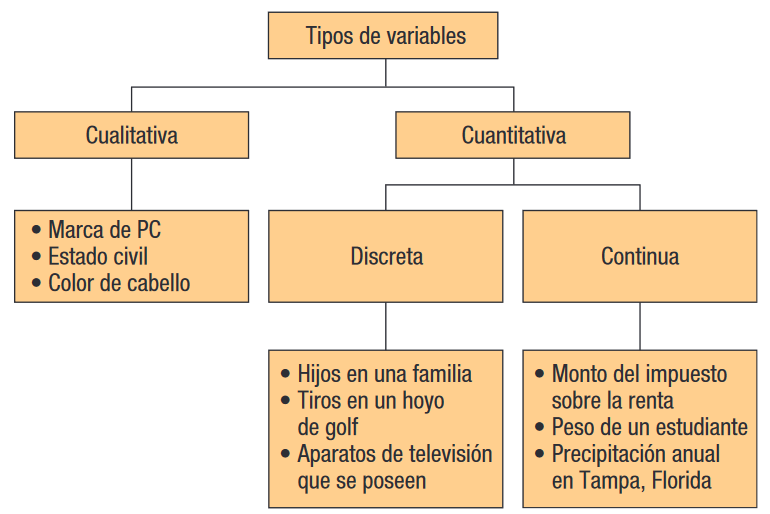
\includegraphics[width=14cm, height=8cm]{resumenTiposVariables1_2}

\subsection{Niveles de medición.}
Los datos se clasifican por niveles de medición. El nivel de medición de los datos rige los cálculos que se llevan a cabo con el fin de resumir y presentar los datos. También determina las pruebas estadísticas que se deben realizar. De hecho, existen cuatro niveles de medición: nominal, ordinal, de intervalo y de razón. La medición mas baja, o mas primaria, corresponde al nivel nominal. La mas alta, o el nivel que proporciona la mayor información relacionada con la observación, es la medición de razón.

\subsubsection*{Datos de nivel nominal.}
Las observaciones acerca de una variable cualitativa solo se clasifican y se cuentan. No existe una forma particular para ordenar las etiquetas, no existe un orden natural. Para el nivel nominal, la medición consiste en contar, a veces, para una mejor compresión de lectura, estos conteos se convierten en porcentajes. Es necesario hacer que el porcentaje sume un total de 100\%, no existe un orden natural para los resultados. Para procesar datos a menudo se codifica la información en forma numérica. El nivel nominal tiene las siguientes propiedades:
\begin{enumerate}
	\item La variable de interés se divide en categorías o resultados.
	\item No existe un orden natural de los resultados.
	\item Los datos solo se clasifican.
\end{enumerate}

\subsubsection*{Datos de nivel ordinal.}
El nivel inmediato superior de datos es el \textbf{nivel ordinal}. No es posible distinguir la magnitud de las diferencias entre los grupos, ¿la diferencia entre superior y bueno es la misma que entre lo malo e inferior? No es posible afirmarlo. Las propiedades del nivel ordinal de los datos son las siguientes:
\begin{enumerate}
	\item Las clasificaciones de los datos se encuentran representadas por conjuntos de etiquetas o nombre (alto, medio, bajo), las cuales tienen valores relativos.
	\item En consecuencia, los valores relativos de los datos se pueden clasificar u ordenar.
\end{enumerate}

\subsubsection*{Datos de nivel de intervalo.}
\textbf{El nivel de intervalo} de medición es el nivel inmediato superior. Incluye todas las características de nivel ordinar, pero, ademas, la diferencia entre valores constituye una magnitud constante. Si las distancias entre los números tienen sentido, aunque las razones no, entonces tiene una escala de intervalo de medición. Las propiedades de los datos de nivel intervalo son las siguientes:
\begin{enumerate}
	\item Las clasificaciones de datos se ordenan de acuerdo con el grado que posea de las característica en cuestión.
	\item Diferencias iguales en la característica representan diferencias iguales en las mediciones (es decir la diferencia entre valores es significativa).
	\item El cero es relativo (no indica ausencia de estado).
\end{enumerate}

\subsubsection*{Datos de nivel de razón.}
Todos los datos cuantitativos son registrados en el nivel de razón de la medición, el \textbf{nivel de razón} es el \textit{mas alto}. Posee todas las características del nivel de intervalo, aunque, ademas, el punto 0 tiene sentido y la razón entre dos números significativa, si se encuentra en 0 significa la ausencia de algo (peso, dinero, etc). Las propiedades de los datos de nivel intervalo son las siguientes:
\begin{enumerate}
	\item Las clasificaciones de datos se ordenan de acuerdo con la cantidad de características que poseen.
	\item Diferencias iguales en la característica representan diferencias iguales en los números asignados a las clasificaciones.
	\item El punto cero representa la ausencia de características y la razón entre dos números es significativa.
	\item La razón entre valores es significativa.
\end{enumerate}
La siguiente grafica resume las principales características de los diversos niveles de medición.
\\
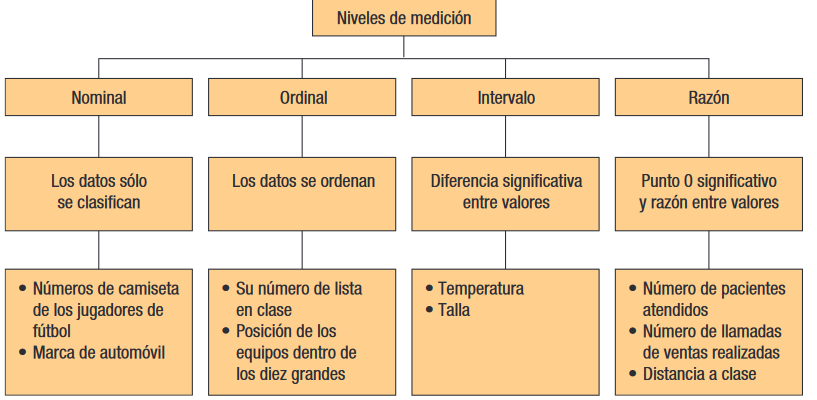
\includegraphics[width=16cm, height=8cm]{resumenCaracteristicasNivelesMedicion1_3}
\section{Capitulo 2. Descripción de datos: tablas de frecuencias, distribuciones de frecuencias y su representación grafica.}
\subsection{Descripción de datos.}
{\large Tabla de frecuencias, distribuciones de frecuencias y su representación grafica.}
\subsection{Construcción de una tabla de frecuencias.}
La estadística descriptiva se encarga de organizar datos con el fin de mostrar la distribución general de estos y el lugar en donde tienden concentrarse, ademas de señalar valores de datos pocos usuales o extremos. El primer procedimiento que se emplea para organizar y resumir un conjunto de datos es una \textbf{tabla de frecuencias.}
\begin{center}
	\textbf{Tabla de frecuencias:} Agrupación de datos cualitativos en clases mutuamente excluyentes que muestra el numero de observaciones en cada clase.
\end{center}
Recordar que, una variable cualitativa es de naturaleza no numérica; es decir, que la información es clasificable en distintas categorías. No hay un orden particular en estas categorías. Por otro lado, están las variables cuantitativas son de índole numérica.
\subsubsection*{Frecuencias relativas de clase.}
Es posible convertir las frecuencias de clase en frecuencias relativas de clase para mostrar la fracción del numero total de observaciones en cada una de ellas. Una frecuencia relativa capta la relación entre la totalidad de elementos de una clase y el numero total de observaciones. Para convertir una distribución de frecuencias en una distribución de frecuencias relativa, cada una de las frecuencias de clase se divide entre el total de observaciones.

\subsubsection*{Representación grafica de datos cualitativos.}
El instrumento mas común para representar una variable cualitativa en forma grafica es la \textbf{grafica de barras}. En la mayoría de los casos, el eje horizontal muestra la variable de interés y el eje vertical la frecuencia o fracción de cada uno de los posibles resultados. Una característica distinta de esta herramienta es que existe una distancia o espacio entre las barras. Una grafica de barras es una representación grafica de una tabla de frecuencias mediante una serie de rectángulos de anchura uniforme, cuya altura corresponde a la frecuencia de clase.
\begin{center}
	\textbf{Grafica de barras:} En ella, las clases se representan en el eje horizontal y la frecuencia de clase en el eje vertical. Las frecuencias de clase son proporcionales a las alturas de las barras.
\end{center}
Se muestra ejemplo de una grafica de barras en la siguiente pagina:\\
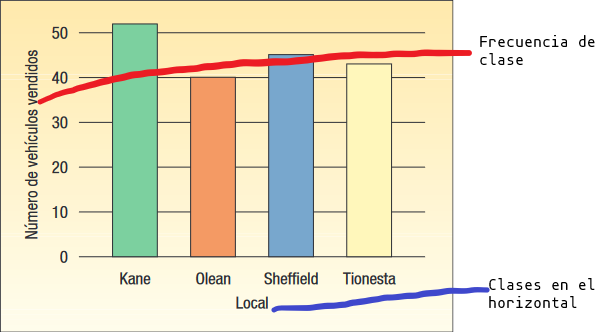
\includegraphics[width=13cm]{graficaBarras2_1.png} \\
Otro tipo de grafica útil para describir información cualitativa es la \textbf{grafica de pastel}.
\begin{center}
	\textbf{Grafica de pastel: }Grafica que muestra la parte o porcentaje que representa cada clase del total de números de frecuencia.
\end{center}
El primer paso para elaborar una grafica de pastel consiste en registrar los porcentajes 0, 5, 10, 15, etc, de manera uniforme alrededor de la circunferencia de un circulo. El área rebanada representa alguna clase, cada rebanada de pastel representa la  porción relativa de cada componente, es posible compararlas con facilidad.\\
Acá un ejemplo de grafica bizcochuelo.\\
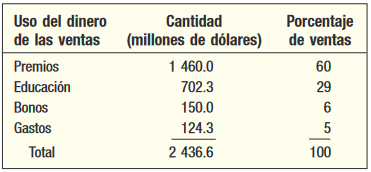
\includegraphics{tablaFrecuenciasRelativas2_2.PNG}\\
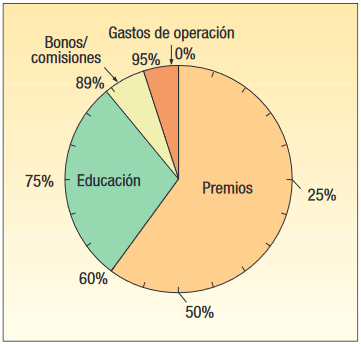
\includegraphics[width=12cm, height=10cm]{graficoPastel2_2.png} \\
Las graficas de pastel y las de barras cumplen casi la misma función. ¿Cuales son los criterios para elegir una u otra? En la mayoría de los casos, las graficas de pastel son las mas informativas cuando se trata de comparar la diferencia relativa en el porcentaje de observaciones de cada uno de las variables de la escala nominal. Es preferible usar una grafica de barras cuando el objetivo es comparar el numero de observaciones en cada categoría.
\subsection{Construcción de distribuciones de frecuencias: datos cuantitativos.}
Distribución de frecuencias puede ser útil para describir la ganancias de ventas.
\begin{center}
	\textbf{Distribución de frecuencias: }Agrupación de datos en clases mutuamente excluyentes, que muestra el numero de observaciones que hay en cada clase.
\end{center}
¿Como crear una distribución de frecuencias? El primer paso consiste en acomodar los datos en una tabla que muestre las clases y el numero de observaciones que hay en cada clase. Recordá que el \textbf{objetivo} es construir tablas, diagramas y graficas que revelen rápidamente la concentración, los valores extremos y la distribución de los datos.
La información desorganizada como \textbf{datos en bruto} o \textbf{datos no agrupados}. Los datos en bruto se interpretan con mayor facilidad si se organizan como una distribución de frecuencias.\\
\textbf{Paso 1: Defina el numero de clases.} El objetivo consiste en emplear suficientes agrupamientos o \textbf{clases}, de manera tal que se perciba la forma de la distribución. Acá se necesita criterio. Una gran cantidad de clases o muy pocas podrían no permitir ver la conformación fundamental del conjunto datos. Una receta útil para determinar la cantidad de clases $(k)$ es la regla de 2 a la $k$. Esta guiá sugiere que se elija el menor numero $ (k) $ para el numero clases, de tal manera que $ 2^{k} $ sea mayor que el numero de observaciones $ (n) $. Ejemplo $ n=180 $ observaciones, si supone $ k=7 $, lo cual significa que utilizara siete clases, entonces $ 2^{7}=128 $, algo menos que las 180 observaciones. De ahí que 7 no represente suficientes clases. Si $ k=8 $, entonces $ 2^{8}=256$, que es mayor 180. Por lo tanto, el numero de clases se recomienda es de 8. \\\\
\textbf{Paso 2: Determine el intervalo o ancho de clase.} El \textbf{intervalo} o \textbf{ancho de clase} debería ser el mismo para todas las clases. Todas las clases juntas deben cubrir por lo menos la distancia del valor mas bajo al mas alto de los datos. Expresado esto en una formula seria:
\[ i\geq \frac{H-L}{k} \]
Por lo general el tamaño de intervalo se redondea a una cifra conveniente, tal como un múltiplo de 10 a 100. En las distribuciones de frecuencia son preferibles los intervalos de clase iguales. Sin embargo, en ciertos casos se necesita que no lo sean para evitar una gran cantidad de clases vacías, o casi vaciás.\\\\

\textbf{Paso 3: Establezca los limites de cada clase.} Este paso es importante para que sea posible incluir cada observación en una sola categoría. Esto significa que debe evitar la superposición de limites de clase confusos. Por ejemplo, clases como \$1300 - \$1400 y \$1400 - \$1500 no deberían emplearse porque no resulta claro si el valor de \$1400 pertenece a la primera o a la segunda clases. Las clases como \$1300 - \$1400 y \$1500 - \$1600 se emplean con frecuencia, aunque también pueden resultar confusas si no se conviene en redondear todos los datos de \$1450 o por arriba de esta cantidad a la segunda clase y los datos por debajo de \$1400 a la primera clase. Al redondear el intervalo de clase hacia arriba con el fin de obtener un tamaño conveniente de clase, se cubre un rango mas amplio que el necesario. Una directriz consiste en convertir el limite inferir de la primera clase en un múltiplo del intervalo de clase. A veces esto no es posible, pero el limite inferior por lo menos debe redondearse.\\\\
\textbf{Paso 4: Anote las veces que encuentre las observaciones en el intervalo en las clases.}  \textbf{PONER IMAGEN PASO 4}
\\\\\textbf{Paso 5: Cuente el numero de elementos de cada clase.}  El numero de elementos que hay en cada clase recibe el nombre de \textbf{frecuencia de clase.} Por ejemplo en numero de \$200 a \$600 hay 8 observaciones, y en la clase de \$600 a \$1000 hay 11 observaciones. Por lo tanto la frecuencia de clase de la primera es de 8, mientras que en la segunda es de 11. Hay un total de 180 observaciones o frecuencias en todo el conjunto de datos. así que la suma de todas las frecuencias debe ser igual a 180. \textbf{PONER TABLA2-7}\\\\
Con frecuencia aparecerán otros dos términos: \textbf{punto medio de clase} e \textbf{intervalo de clase.} El punto medio, que se encuentra entre los limites inferiores de dos clases consecutivas, se calcula sumando los limites interiores de clases consecutivas y dividiendo el resultado entre dos. En caso de la imagen del paso 5, el limite de clase interior de la primera clase es de \$200 y el siguiente limite es de \$600. El punto medio de clase \$400, que se calcula mediante la operación \[ \frac{\$600+\$200}{2} .\] El punto medio de \$400 representa mejor. Para determinar el intervalo de clase, se resta el limite inferior de la clase del limite inferior de la siguiente clase, es decir \[ \$600 -\$200 =400.\]Cambien se puede determinar el intervalo de clase calculando la diferencia entre puntos medios consecutivos. El punto medio de la primera clase des de \$400 y el punto medio de la segunda clase es de \$800. La diferencia es de \$400.
\subsection{Distribución de frecuencias relativas}
Si se requiere resumir las ventas del ultimo mes utilizando ganancia por venta; seria útil describir la ganancia de venta por medio de una distribución de frecuencias.
\begin{center}
	\textbf{Distribución de frecuencias: }Agrupación de datos en clases mutuamente excluyentes, que muestra el numero de observaciones que hay en cada clase.
\end{center}
¿Como crear una distribución de frecuencias? El primer paso consiste en acomodar los datos en una tabla que muestre las clases y el numero de observaciones que hay en cada clase. El objetivo es construir tablas, diagramas y graficas que revelen rápidamente la concentración, los valores extremos y la distribución de los datos. La información desorganizada como \textbf{datos en bruto} o \textbf{datos no agrupados.} Los datos en bruto se interpretan con mayor facilidad si se organizan como una distribución de frecuencias.\\\\
\textbf{Paso 1: Defina el numero de clases: }El objetivo consiste en emplear suficientes agrupamientos o \textbf{clases}, de manera tal que se perciba la forma de la distribución. Se necesita criterio. Una gran cantidad de clases o muy pocas podrían no permitir ver la conformación fundamental del conjunto de datos. Una receta útil para determinar la cantidad de clases (k) es la regla de 2 a la k. Esta guía sugiere que se elija el menor numero (k) para el numero de clases, de tal manera que \[2^{k}\] sea mayor que el numero de observaciones (n). Si $ n=180 $, si supone que $ k=7 $, lo cual significa que utilizara siete clases, entonces \[ 2^{7}=128 \], algo menos de 180. De ahí que 7 no represente suficiente clases. Si $ k=8 $, entonces \[ 2^{8}=256 \], que es mayor a 180. Por lo tanto, el numero de clases que se recomienda es de 8.\\\\
\textbf{Paso 2: Determine el intervalo o ancho de clase:} El \textbf{intervalo o ancho de clase} debería ser el mismo para todas las clases. Todas las clases juntas deben cubrir por lo menos la distancia del valor mas bajo al mas alto de los datos. Expresado esto en una formula seria: \[ i\geq\frac{H-L}{k} \] en la que la $ i $ es el intervalo de clase; H, el máximo valor observado; L, el mínimo valor observado, y k, el numero de clases. En la practica, por lo general este tamaño de intervalo se redondea a una cifra conveniente, tal como un múltiplo de 10 a 100. Las distribuciones de frecuencia son preferibles los intervalos de clase iguales. Ciertos casos se necesita que no lo sean para evitar una gran cantidad de clases vacías, o casi vacías. Facilita la compresión de la información.\\\\
\textbf{Paso 3: Establezca los limites de cada clase:} Este paso es importante para que esa posible incluir cada observación en una sola categoría. Esto significa que debe evitar la superposición de limites de clase confusos. Ponele tenes una clase 200-400 y otra de 400-600 ¿el 400 va incluido en la primera clase o en la segunda clase? ACLARA ESO O NO ENTIENDO NADADORA.\\\\
\textbf{Paso 4: Anote las observaciones en las clases:} Se da un ejemplo en la imagen siguiente \textbf{AGREGAR TABLA DEL PASO 4}\\\\
\textbf{Paso 5: Cuente el numero de elementos de cada clase:} El numero de elementos que hay en cada clase recibe el nombre \textbf{frecuencia de clase.} En la clase \$200 a \$600 hay 8 observaciones, y en la clase de \$600 a \$1000 hay 11 observaciones. Por lo tanto, la frecuencia de clase de la primera clase es de 8, mientras que en la segunda es de 11. Hay un total de 180 observaciones o frecuencias en todo el conjunto de datos. Así que la suma de todas las frecuencias debe ser igual a 180. \textbf{PEGAR TABLA2-7}
Las ventajas de condesar los datos de forma mas entendible y organizada compensa por mucho este desventaja. \linebreak[2]
Con frecuencia aparecerán otros dos términos: \textbf{punto medio de clase e intervalo de clase}. El punto medio, que se encuentra los limites inferiores de dos clases consecutivos, se calcula sumando los limites inferiores de clases consecutivas y dividiendo el resultado entre dos. Para determinar el intervalo de clase, se resta el limite inferior de la clase del limite inferior de la siguiente clase.
\subsection{Distribución de frecuencias relativas.}
Convertir frecuencias de clase en frecuencias relativas de clase, igual que con los datos cualitativos, con el fin de mostrar la fracción del total de observaciones que hay en cada clase. Una distribución de frecuencias relativas convierte la frecuencia en un porcentaje. Para convertir una distribución de frecuencia en una distribución de frecuencia relativa, cada una de las frecuencias de las clases se divide entre el numero total de observaciones. A continuación dejo la tabla de como serian una frecuencia relativa. \textbf{PONER TABLA 2-8}
\subsection{Representación grafica de una distribución de frecuencias.}
Es frecuente que se necesite una vista rápida de las tendencias de las ventas, los precios de las acciones o costos de hospitalización. A menudo, estas tendencias se describen por medio de tablas y graficas. Tres herramientas que serán de utilidad para representar gráficamente una distribución de frecuencias son el histograma, el polígono de frecuencias y el polígono de frecuencias acumuladas.
\subsubsection*{Histograma}
Un histograma de una distribución de frecuencias basadas en datos cuantitativos se asemeja mucho a la grafica de barras, que muestra la distribución de datos cualitativos. Las clases se señalan en el eje horizontal y las frecuencias de clase en el eje vertical. Las frecuencias de clase se representan por medio de las alturas de las barras. Existe una importante diferencia como consecuencia de la naturaleza de los datos. Por lo general, los datos cuantitativos se miden con escalas continuas, no discretas. Por lo tanto, el eje horizontal representa todos los valores posibles y las barras se colocan de forma adyacente para que muestren la naturaleza continua de los datos.
\begin{center}
	\textbf{Histograma: }Grafica en la que las clases se señalan en el eje horizontal y las frecuencias de clase en el eje vertical. Las frecuencias de clase se representan por medio de las altura de las barras, que se dibujan de manera adyacente.
\end{center}
Mostraremos un ejemplo a continuación.
\subsubsection*{Poligono de frecuencias}
Un polígono de frecuencias también muestra la forma que tiene una distribución y es similar a un histograma. Consiste en segmentos de recta que conectan los puntos que forman las intersecciones de los puntos medios de clase y frecuencias de clase. El punto medio de cada clase se indica en una escala en el eje X y las frecuencias de clase en el Y. Recordá que el punto medio de clase es el valor localizado en el centro de una clase y representa los valores típicos de ella (limite superior - limite inferior). La frecuencia de clase es el numero de observaciones que hay en una clase particular. Para construir un polígono de frecuencias, hay que desplazarse horizontalmente sobre la grafica al punto medio, y en seguida de manera vertical, la frecuencia de clase, donde se coloca un punto. Los valores X y de Y de este punto reciben el nombre de \textit{coordenadas}. El proceso continua con todas las clases. Posteriormente, los puntos se conectan de manera ordenada. Es decir, que el punto que representa la clase mas baja se une al que representa la segunda clase y así en lo sucesivo. \textbf{PONER GRAFICA 2-5}\linebreak Tanto el histograma como el polígono de frecuencias permiten tener una vista rápida de las principales características de los datos (máximos, mínimos, puntos de concentración, etc.). Aunque las dos representaciones tienen un propósito similar, el histograma posee la ventaja de que describe cada clase como un rectángulo, en el que la barra de altura de este representa el numero de elementos que hay en cada clase. El polígono de frecuencias, en cambio, tiene una ventaja con respecto al histograma. También permite comparar directamente dos o mas distribuciones de frecuencias \textbf{PONER GRAFICA 2-6 DE EJEMPLO}.
\subsubsection*{Distribuciones de frecuencia acumulativas}.
Una distribución de frecuencias acumulativas muestra el numero o porcentaje de observaciones por debajo de valores dados, con representación gráfica de un \textbf{polígono de frecuencias acumulativas.} Como su nombre lo indica, una distribución de frecuencias acumulativas y un polígono de frecuencias acumulativas implican \textit{frecuencias acumulativas}. La frecuencia acumulativa básicamente vas sumando todas las frecuencias de las clases. \textbf{PONER TABLA 2-9}
Para trazar una distribución de frecuencias acumulativas, \textbf{se ubica el limite superior de cada clase en una escala a lo largo del eje X}, y \textbf{las correspondientes frecuencias acumulativas, a lo largo del eje Y}. Para incluir información adicional, gradué el eje vertical a la izquierda en unidades y el eje vertical a la derecha en porcentajes.
\section{Capitulo 3. Descripción de datos: medidas numéricas.}
\subsection{Introducción}
En este capitulo se presentan dos formas numéricas de describir datos cuantitativos: las \textbf{medidas de ubicación} y las \textbf{medidas de dispersión.} A las medidas de ubicación a menudo se les llama promedios. El propósito de una medida de ubicación consiste en señalar el centro de un conjunto de valores. Vos ya estas conoces el concepto de promedio (media aritmética), medida de ubicación que muestra el valor central de los datos. Si solo tomas las medidas de ubicación en cuenta de un conjunto de datos o si compara varios conjuntos de datos utilizando valores centrales, llegara a una conclusión incorrecta. Ademas de las medidas de ubicación, debe tomar en consideración la \textbf{dispersión} (con frecuencia se le llama \textit{frecuencia variación }o \textit{propagación}) de los datos. Para describir la dispersión considere el rango, la desviación media, la varianza y la desviación estándar. En principio se explican las medidas de ubicación. No existe una única medida de dispersión; de hecho existen varias. Consideraremos cinco:
\begin{enumerate}
	\item La media aritmética.
	\item La media ponderada.
	\item La mediana.
	\item La moda.
	\item La media geométrica.
\end{enumerate}
La medida aritmética es la medida de ubicación que mas se utiliza y que se publica con mayor frecuencia, por lo cual se le considerará como parámetro para una población y como estadístico para las muestras.
\subsection{La media poblacional}
La media poblacional es la suma de todos los valores observados en la población dividida entre el numero de valores de la población. Para determinar la media poblacional, aplique la siguiente formula con símbolos matemáticos:
\[ \mu=\frac{\sum X}{N} \] 
En la cual:
\begin{enumerate}
	\item $\mu$ representa la media poblacional; se trata de la letra minúscula griega mu.
	\item $N$ es la numera de valores en la población.
	\item $X$ representa cualquier valor particular.
	\item $\sum$ es la letra mayúscula griega sigma e indica la operación de suma.
	\item $\sum X$ es la suma de X valores en la población.
\end{enumerate}
hola mundo
\end{document}
